%%%%%%%%%%%%%%%%%%%%%%%%%%%%%%%%%%%%%%%%%
% Masters/Doctoral Thesis 
% LaTeX Template
% Version 1.43 (17/5/14)
%
% This template has been downloaded from:
% http://www.LaTeXTemplates.com
%
% Original authors:
% Steven Gunn 
% http://users.ecs.soton.ac.uk/srg/softwaretools/document/templates/
% and
% Sunil Patel
% http://www.sunilpatel.co.uk/thesis-template/
%
% License:
% CC BY-NC-SA 3.0 (http://creativecommons.org/licenses/by-nc-sa/3.0/)
%
% Note:
% Make sure to edit document variables in the Thesis.cls file
%
%%%%%%%%%%%%%%%%%%%%%%%%%%%%%%%%%%%%%%%%%

%----------------------------------------------------------------------------------------
%	PACKAGES AND OTHER DOCUMENT CONFIGURATIONS
%----------------------------------------------------------------------------------------

\documentclass[11pt, oneside]{Thesis} % The default font size and one-sided printing (no margin offsets)

\graphicspath{{images/}} % Specifies the directory where pictures are stored

%\usepackage[round, comma, sort&compress]{natbib} % Use the natbib reference package - read up on this to edit the reference style; if you want text (e.g. Smith et al., 2012) for the in-text references (instead of numbers), remove 'numbers' 
\hypersetup{urlcolor=blue, colorlinks=true} % Colors hyperlinks in blue - change to black if annoying

\usepackage{amsmath,amsfonts,amssymb}

\usepackage{epsfig}

\usepackage{lineno}
\usepackage{ltablex}

\usepackage[tight,footnotesize]{subfigure}

 
\usepackage{multirow}
%\usepackage[english,algoruled,vlined]{algorithm2e}
\usepackage{algorithm}
\usepackage{algpseudocode}
\usepackage{amsmath}
%\usepackage{hyperref}
\usepackage{minitoc}
%\setcounter{secnumdepth}{1}% number \part and \chapter in book classes
\usepackage{array}
\usepackage{xparse}
\usepackage{tabularx}

\usepackage{listings}
%Define the HATP language
%
%Author: Raphaël Lallement, raphael . lallement [at] laposte . net

\usepackage{listings}

\lstdefinelanguage{HATP}{
	keywords={define,entityType,entityAttributes,
		dynamic,static,atom,set,bool,string,number,
		true,false,NULL,new,add,in,rem,
		method,operator,projects,preconditions,effects,cost,duration,subtasks,goal,
		FORALL,EXIST,IF,SELECT,SELECTONCE,SELECTORDERED, plans},
	sensitive=true,
	comment=[l]{//},
	string=[b]{"},
	tabsize=3,
	basicstyle={\singlespacing},aboveskip={-3ex}
}

\lstalias{hatp}{HATP}
 


\title{\ttitle} % Defines the thesis title - don't touch this

\begin{document}

\frontmatter % Use roman page numbering style (i, ii, iii, iv...) for the pre-content pages

\setstretch{1.3} % Line spacing of 1.3

% Define the page headers using the FancyHdr package and set up for one-sided printing
\fancyhead{} % Clears all page headers and footers
\rhead{\thepage} % Sets the right side header to show the page number
\lhead{} % Clears the left side page header

\pagestyle{fancy} % Finally, use the "fancy" page style to implement the FancyHdr headers

\newcommand{\HRule}{\rule{\linewidth}{0.5mm}} % New command to make the lines in the title page

\theoremstyle{plain}
\newtheorem*{prop}{Assumption}

\makeatletter
\newcommand{\thickhline}{%
    \noalign {\ifnum 0=`}\fi \hrule height 1.5pt
    \futurelet \reserved@a \@xhline
}
\newcolumntype{"}{@{\hskip\tabcolsep\vrule width 1.5pt\hskip\tabcolsep}}
\makeatother


% PDF meta-data
\hypersetup{pdftitle={\ttitle}}
\hypersetup{pdfsubject=\subjectname}
\hypersetup{pdfauthor=\authornames}
\hypersetup{pdfkeywords=\keywordnames}

\linenumbers % to activate the line numbers
\renewcommand\thelinenumber{\color{red}\arabic{linenumber}}

%----------------------------------------------------------------------------------------
%	TITLE PAGE
%----------------------------------------------------------------------------------------

\begin{titlepage}
\begin{center}

\textsc{\LARGE \univname}\\[1.5cm] % University name
\textsc{\Large Doctoral Thesis}\\[0.5cm] % Thesis type

\HRule \\[0.4cm] % Horizontal line
{\huge \bfseries \ttitle}\\[0.4cm] % Thesis title
\HRule \\[1.5cm] % Horizontal line
 
\begin{minipage}{0.4\textwidth}
\begin{flushleft} \large
\emph{Author:}\\
\href{http://www.johnsmith.com}{\authornames} % Author name - remove the \href bracket to remove the link
\end{flushleft}
\end{minipage}
\begin{minipage}{0.4\textwidth}
\begin{flushright} \large
\emph{Supervisor:} \\
\href{http://www.jamessmith.com}{\supname} % Supervisor name - remove the \href bracket to remove the link  
\end{flushright}
\end{minipage}\\[3cm]
 
\large \textit{A thesis submitted in fulfilment of the requirements\\ for the degree of \degreename}\\[0.3cm] % University requirement text
\textit{in the}\\[0.4cm]
%\groupname\\\deptname\\[2cm] % Research group name and department name
 
{\large \today}\\[4cm] % Date
%\includegraphics{Logo} % University/department logo - uncomment to place it
 
\vfill
\end{center}

\end{titlepage}

%\newcommand{\todo}[1]{\textbf{\textit{\color{red} #1}}}
%\newcommand{\todo}[1]{#1}
\newcommand{\note}[1]{\textbf{\textit{\color{blue} #1}}}

%----------------------------------------------------------------------------------------
%	DECLARATION PAGE
%	Your institution may give you a different text to place here
%----------------------------------------------------------------------------------------

%\Declaration{
%
%\addtocontents{toc}{\vspace{1em}} % Add a gap in the Contents, for aesthetics

%I, \authornames, declare that this thesis titled, '\ttitle' and the work presented in it are my own. I confirm that:
%
%\begin{itemize} 
%\item[\tiny{$\blacksquare$}] This work was done wholly or mainly while in candidature for a research degree at this University.
%\item[\tiny{$\blacksquare$}] Where any part of this thesis has previously been submitted for a degree or any other qualification at this University or any other institution, this has been clearly stated.
%\item[\tiny{$\blacksquare$}] Where I have consulted the published work of others, this is always clearly attributed.
%\item[\tiny{$\blacksquare$}] Where I have quoted from the work of others, the source is always given. With the exception of such quotations, this thesis is entirely my own work.
%\item[\tiny{$\blacksquare$}] I have acknowledged all main sources of help.
%\item[\tiny{$\blacksquare$}] Where the thesis is based on work done by myself jointly with others, I have made clear exactly what was done by others and what I have contributed myself.\\
%\end{itemize}
% 
%Signed:\\
%\rule[1em]{25em}{0.5pt} % This prints a line for the signature
% 
%Date:\\
%\rule[1em]{25em}{0.5pt} % This prints a line to write the date
%}

\clearpage % Start a new page

%----------------------------------------------------------------------------------------
%	QUOTATION PAGE
%----------------------------------------------------------------------------------------

\pagestyle{empty} % No headers or footers for the following pages

%\null\vfill % Add some space to move the quote down the page a bit
%
%\textit{``Thanks to my solid academic training, today I can write hundreds of words on virtually any topic without possessing a shred of information, which is how I got a good job in journalism."}
%
%\begin{flushright}
%Dave Barry
%\end{flushright}

\vfill\vfill\vfill\vfill\vfill\vfill\null % Add some space at the bottom to position the quote just right

\clearpage % Start a new page

%----------------------------------------------------------------------------------------
%	ABSTRACT PAGE
%----------------------------------------------------------------------------------------

\addtotoc{Abstract} % Add the "Abstract" page entry to the Contents

\abstract{\addtocontents{toc}{\vspace{1em}} % Add a gap in the Contents, for aesthetics
My abstract

\paragraph{Version fran\c caise}
~\\
Mon Abstract
}

\clearpage % Start a new page

%----------------------------------------------------------------------------------------
%	ACKNOWLEDGEMENTS
%----------------------------------------------------------------------------------------

\setstretch{1.3} % Reset the line-spacing to 1.3 for body text (if it has changed)

\acknowledgements{\addtocontents{toc}{\vspace{1em}} % Add a gap in the Contents, for aesthetics

TODO\ldots
}
\clearpage % Start a new page

%----------------------------------------------------------------------------------------
%	LIST OF CONTENTS/FIGURES/TABLES PAGES
%----------------------------------------------------------------------------------------

\pagestyle{fancy} % The page style headers have been "empty" all this time, now use the "fancy" headers as defined before to bring them back


\addtocounter{tocdepth}{-4}% “delete” lowest level from TOC

\lhead{\emph{Contents}} % Set the left side page header to "Contents"
\dominitoc[d]
\setcounter{minitocdepth}{2} 
\tableofcontents % Write out the Table of Contents


\lhead{\emph{List of Figures}} % Set the left side page header to "List of Figures"
\listoffigures % Write out the List of Figures
%
\lhead{\emph{List of Tables}} % Set the left side page header to "List of Tables"
\listoftables % Write out the List of Tables


%----------------------------------------------------------------------------------------
%	ABBREVIATIONS
%----------------------------------------------------------------------------------------
%
\clearpage % Start a new page
%
\setstretch{1.5} % Set the line spacing to 1.5, this makes the following tables easier to read
%
\lhead{\emph{Abbreviations}} % Set the left side page header to "Abbreviations"
\listofsymbols{ll} % Include a list of Abbreviations (a table of two columns)
{
\textbf{MDP} & \textbf{M}arkov \textbf{D}ecision \textbf{P}rocess \\
\textbf{Acronym} & \textbf{W}hat (it) \textbf{S}tands \textbf{F}or \\
}

%----------------------------------------------------------------------------------------
%	PHYSICAL CONSTANTS/OTHER DEFINITIONS
%----------------------------------------------------------------------------------------

%\clearpage % Start a new page
%
\lhead{\emph{Definitions}} % Set the left side page header to "Physical Constants"
%
\begin{itemize}
\item Agent: a human or robot.
\item Entity: an agent, an agent's joint, or an object.
\item Joint: an agent is composed by different joints (e.g. head, hand for a human; gripper, base, for a robot).
\item Action:  a tuple $(name, preconditions, target, postconditions)$. The $name$ of an action is a unique string that identifies it. The $preconditions$ are a list of properties that must be true in order to realize the action. In our system, an action is executed on a $target$, which can be a physical object, like a cup, but also an area of the environment, like a room. The $postconditions$ are the set of properties, and their values, affected by the action's execution.
\item Fact: a statetement composed by a $pubject$, a $predicate$, and a $value$.
\end{itemize}

%----------------------------------------------------------------------------------------
%	SYMBOLS
%----------------------------------------------------------------------------------------
%
%\clearpage % Start a new page
%
%\lhead{\emph{Symbols}} % Set the left side page header to "Symbols"
%
%\listofnomenclature{lll} % Include a list of Symbols (a three column table)
%{
%$a$ & distance & m \\
%$P$ & power & W (Js$^{-1}$) \\
%% Symbol & Name & Unit \\
%
%& & \\ % Gap to separate the Roman symbols from the Greek
%
%$\omega$ & angular frequency & rads$^{-1}$ \\
%% Symbol & Name & Unit \\
%}

%----------------------------------------------------------------------------------------
%	DEDICATION
%----------------------------------------------------------------------------------------

%\setstretch{1.3} % Return the line spacing back to 1.3
%
%\pagestyle{empty} % Page style needs to be empty for this page
%
%\dedicatory{For/Dedicated to/To my\ldots} % Dedication text
%
%\addtocontents{toc}{\vspace{2em}} % Add a gap in the Contents, for aesthetics

%----------------------------------------------------------------------------------------
%	THESIS CONTENT - CHAPTERS
%----------------------------------------------------------------------------------------

\mainmatter % Begin numeric (1,2,3...) page numbering

\pagestyle{fancy} % Return the page headers back to the "fancy" style

% Include the chapters of the thesis as separate files from the Chapters folder
% Uncomment the lines as you write the chapters

\setcounter{mtc}{5}


\addtocontents{toc}{\vspace{2em}} % Add a gap in the Contents, for aesthetics


\newpage


\setcounter{mtc}{5}
% Chapter Template

\chapter{Introduction} % Main chapter title

\label{chapter-introduction} % Change X to a consecutive number; for referencing this chapter elsewhere, use \ref{ChapterX}

\lhead{Chapter . \emph{Introduction}} % Change X to a consecutive number; this is for the header on each page - perhaps a shortened title

%----------------------------------------------------------------------------------------
%	SECTION 1
%----------------------------------------------------------------------------------------

In the current days robots are starting to be introduced in our lives more and more, and we can expect that, in the next years, they will complete the transition from mechanic tools, used mostly in industries, to true partners and companions. There is an increasing interest in studying how robots should behave in environments inhabited by humans, and in some works robots have been deployed in crowded and dynamic environments, like airports and museums.

Human-Robot cooperation poses a multitude of problems. Imagine a mobile robot working in a warehouse, carrying and sorting crates in different locations. Already, we are presented with quite a complex problem, where the robot needs to have a good representation of the world (i.e. position of the crates, obstacles, layout of the warehouse), to create plans to reach the goal (which crates to move, where to bring them, which paths to follow), and to have sufficient motion and manipulation skills to achieve them. If humans are present in the environment, they should be represented and considered by the robot in its plans and actions.  Modeling humans as simple moving obstacles might not be enough if we consider issues of trust, legibility, and acceptability. The robot should respect a number of social rules in the presence of humans, like maintaining a socially acceptable distance, whenever possible, from them, and approaching them from a visible positions.

The problem becomes even more complex when robots and humans need to cooperate to solve a goal, for example by sorting together the crates, or even by sharing the load of heavy objects. To understand  how to approach this problem we can observe how humans cooperate with themselves. Psychological and philosofical research \cite{pacherie2012phenomenology} characterizes the execution of cooperative actions as 'joint actions'. Sebanz et al. \cite{sebanz2006joint} have proposed that the execution of a joint action depends on three different abilities: sharing representations, predicting actions, and integrating predicted effects of own and other's actions. These abilities can be achieved by the combination of different mechanisms:
\begin{itemize}
\item Joint Attention. The ability to direct a partner's attention, in order to create a shared representation of objects and events. Humans use a large number of social cues, like gaze direction or pointing gestures, to indicate what is currently under observation. This mechanism helps filling important gaps in the knowledge of a partner, and points to the importance of understanding what others know and perceive.
\item Action Observation: observing other partners' actions is crucial in understanding what are their goals. Studies have shown that observing a person performing an action produces a motor resonance, which increases with the observer's level of expertise in the action. Understanding what others are doing allows to predict the outcomes of their activities, and even their next movements.
\item Task Sharing: humans are able to predict, in some circumstances, what others will do  even without direct observation. A notable example is a well trained sport team, which is able to act like a single entity, coordinating seamlessly. This ability suggests that humans possess a shared representation of tasks, which include actions that should be performed by each partner of the team.
\item Action Coordination: predicting actions is not enough. Humans also need to choose a complementary action, and adjusting its parameters, like the exact moment and place where it should be performed, to partners. 
\end{itemize}

It seems that robots need to have an equivalent of these mechanism, in order to cooperate in a natural and acceptable way with humans. Is this enough to include robots in our lives? Unfortunately, we just scratched the surface of the problem. While these areas are already very complex, and not completely understood, humans possess other skills, that should be translated to robots. For example, when a robot's behavior shows a degree of intelligence, humans usually try to have a conversation with it, which can lead to frustation, or often disbelief in the actual capacities of the robot. Issues such as dialogue, representation and refinement of knowledge are very complex and will be a direct focus of this work.

The goal of this thesis is, instead, to provide a framework to allow a robot to work in social environments and execute joint actions with humans in a natural way. We built our system using psychology as an inspiration, without trying to replicate accurately human mechanism, an area of work studied in cognitive systems. 

There are still not many robotic architecture that take humans into account at all levels, from planifications to execution. We will review some examples:
\begin{itemize} 
\item \cite{trafton2013act} presents ACT-R/E, a cognitive architecture, based
on the ACT-R architecture, used for human robot interaction tasks. The
architecture aims at simulating how humans think, perceive and act in
the world. ACT-R/E has being tested in different scenarios, such as
theory of mind and hide and seek, to show its capacity of modeling
human behaviors and tought.
\item In \cite{Fong_2006} the authors present  HRI/OS, an agent-based system
that allows humans and robots to work in teams. The system is able to
produce and schedule tasks to different agents, based on their capacities,
and allows the agents to interact mostly in a parallel and independent way, with
loose coordination between them. Cooperation  mainly
takes place when one agent asks for help while
dealing with a situation. In this case the HRI/OS will
look for the best agent to help, based on their availability and capacities.

\item In \cite{clodic2009shary} the authors build SHARY, a supervision
system for human robot interaction, tested in domestic environments to
perform tasks such as serving a drink to a person. Our system is an
evolution of Shary which includes new aspects, like spatial
reasoning and modeling of joint actions.
\end{itemize}

\section{Contributions}

The main contributions of this work are the following:
\begin{itemize}
\item Building a supervision system for human robot interaction, integrating novel algorithms developed in this work with existing, components.
\item Developing a novel algorithm to infer human goals and intentions.
\item Developing a novel probabilistic planning algorithm for multiple agent.
\end{itemize}

\section{System overview}
\label{intro-system_overview}
%TODO: add urls, PR2, GAZEBO, ROS, SPENCER, GTP, Move_Base, Moveit
The supervision system was developed with the following goals:
\begin{itemize}
\item Flexibility. The system is able to work in different scenarios, environments, and different robots.
\item Extendibility. The system can be easily extendable by adding or substituting modules, to introduce different capacities, without having an impact on existing components.
\item Human-Awareness. The system supports human in all its layers. Human belief management, multi-agent planning, human-aware motion and execution, and simple forms of direct interaction are explicitly included in its components.
\end{itemize}

To achieve these goals we use the well-known ROS framework\footnote{http://www.ros.org/}, which naturally supports different robots and modules.The system has been implemented and tested in simulation, using the GAZEBO simulator\footnote{http://gazebosim.org/}, and on two different robots, the PR2 by Willow Garage\footnote{https://www.willowgarage.com/pages/pr2/overview}, and the SPENCER robot\footnote{http://www.spencer.eu/}, developed in an european research project. 

The supervision system is composed by the following layers, as shown in figure \ref{fig:intro-system_architecture}:
\begin{itemize}
\item Situation Assessment. This layer produces symbolic information, using geometrical and temporal reasoning, starting from perception data. Using Situation Assessment, the robot is able to compute information like the reachability of objects, which actions have been performed by humans, and the spatial relationships (distance, orientation, and their variations) between humans and the robot. This layer also includes a Database, which collects collects all the symbolic information produced by the system. The Database is able to represent the knowledge of different agents, as viewed by the robot. Using this feature, the robot can represent, for example, the fact that a human does not know the location of an object, or that he has wrong information about its location.
\item Goal Management. This layer manages the different goals of the robot. Goals can be directly received from exernal inputs, like a human or a terminal, or generated by the robot starting from information present in the Database. For example, after deducing that the human is looking for his glasses in the Situation Assessment Layer, the Goal Management Layer can create a goal to fetch them. 
\item Plan Production and Management. This layer is charged with producing and managing plans to achieve the current goal. The system supports multi-agent plans, and so the robot will monitor other agents' action, to check if they conform to the shared-plan, and interact with the Execution Manager layer to execute the robot's actions. Plans can be managed in three different modalities: robot leader, human leader, and equal partners. Human-Awareness is supported by adapting  production, explanation, and management of plans to the level of experience on the task of the robot's partners. Additionally, this layer supports a simple form of plan negotiation, which allows humans to express preference in the allocation of tasks.
\item Execution Management. This layer handles the execution of the robot's actions, including joint actions shared with other agents. Human safety and robustness are achieved by stopping and resuming operations  when unexpected or dangerous situations arise, like a human moving into the operative area of the robot.
\end{itemize}

 \begin{figure}[h!]
	\centering
	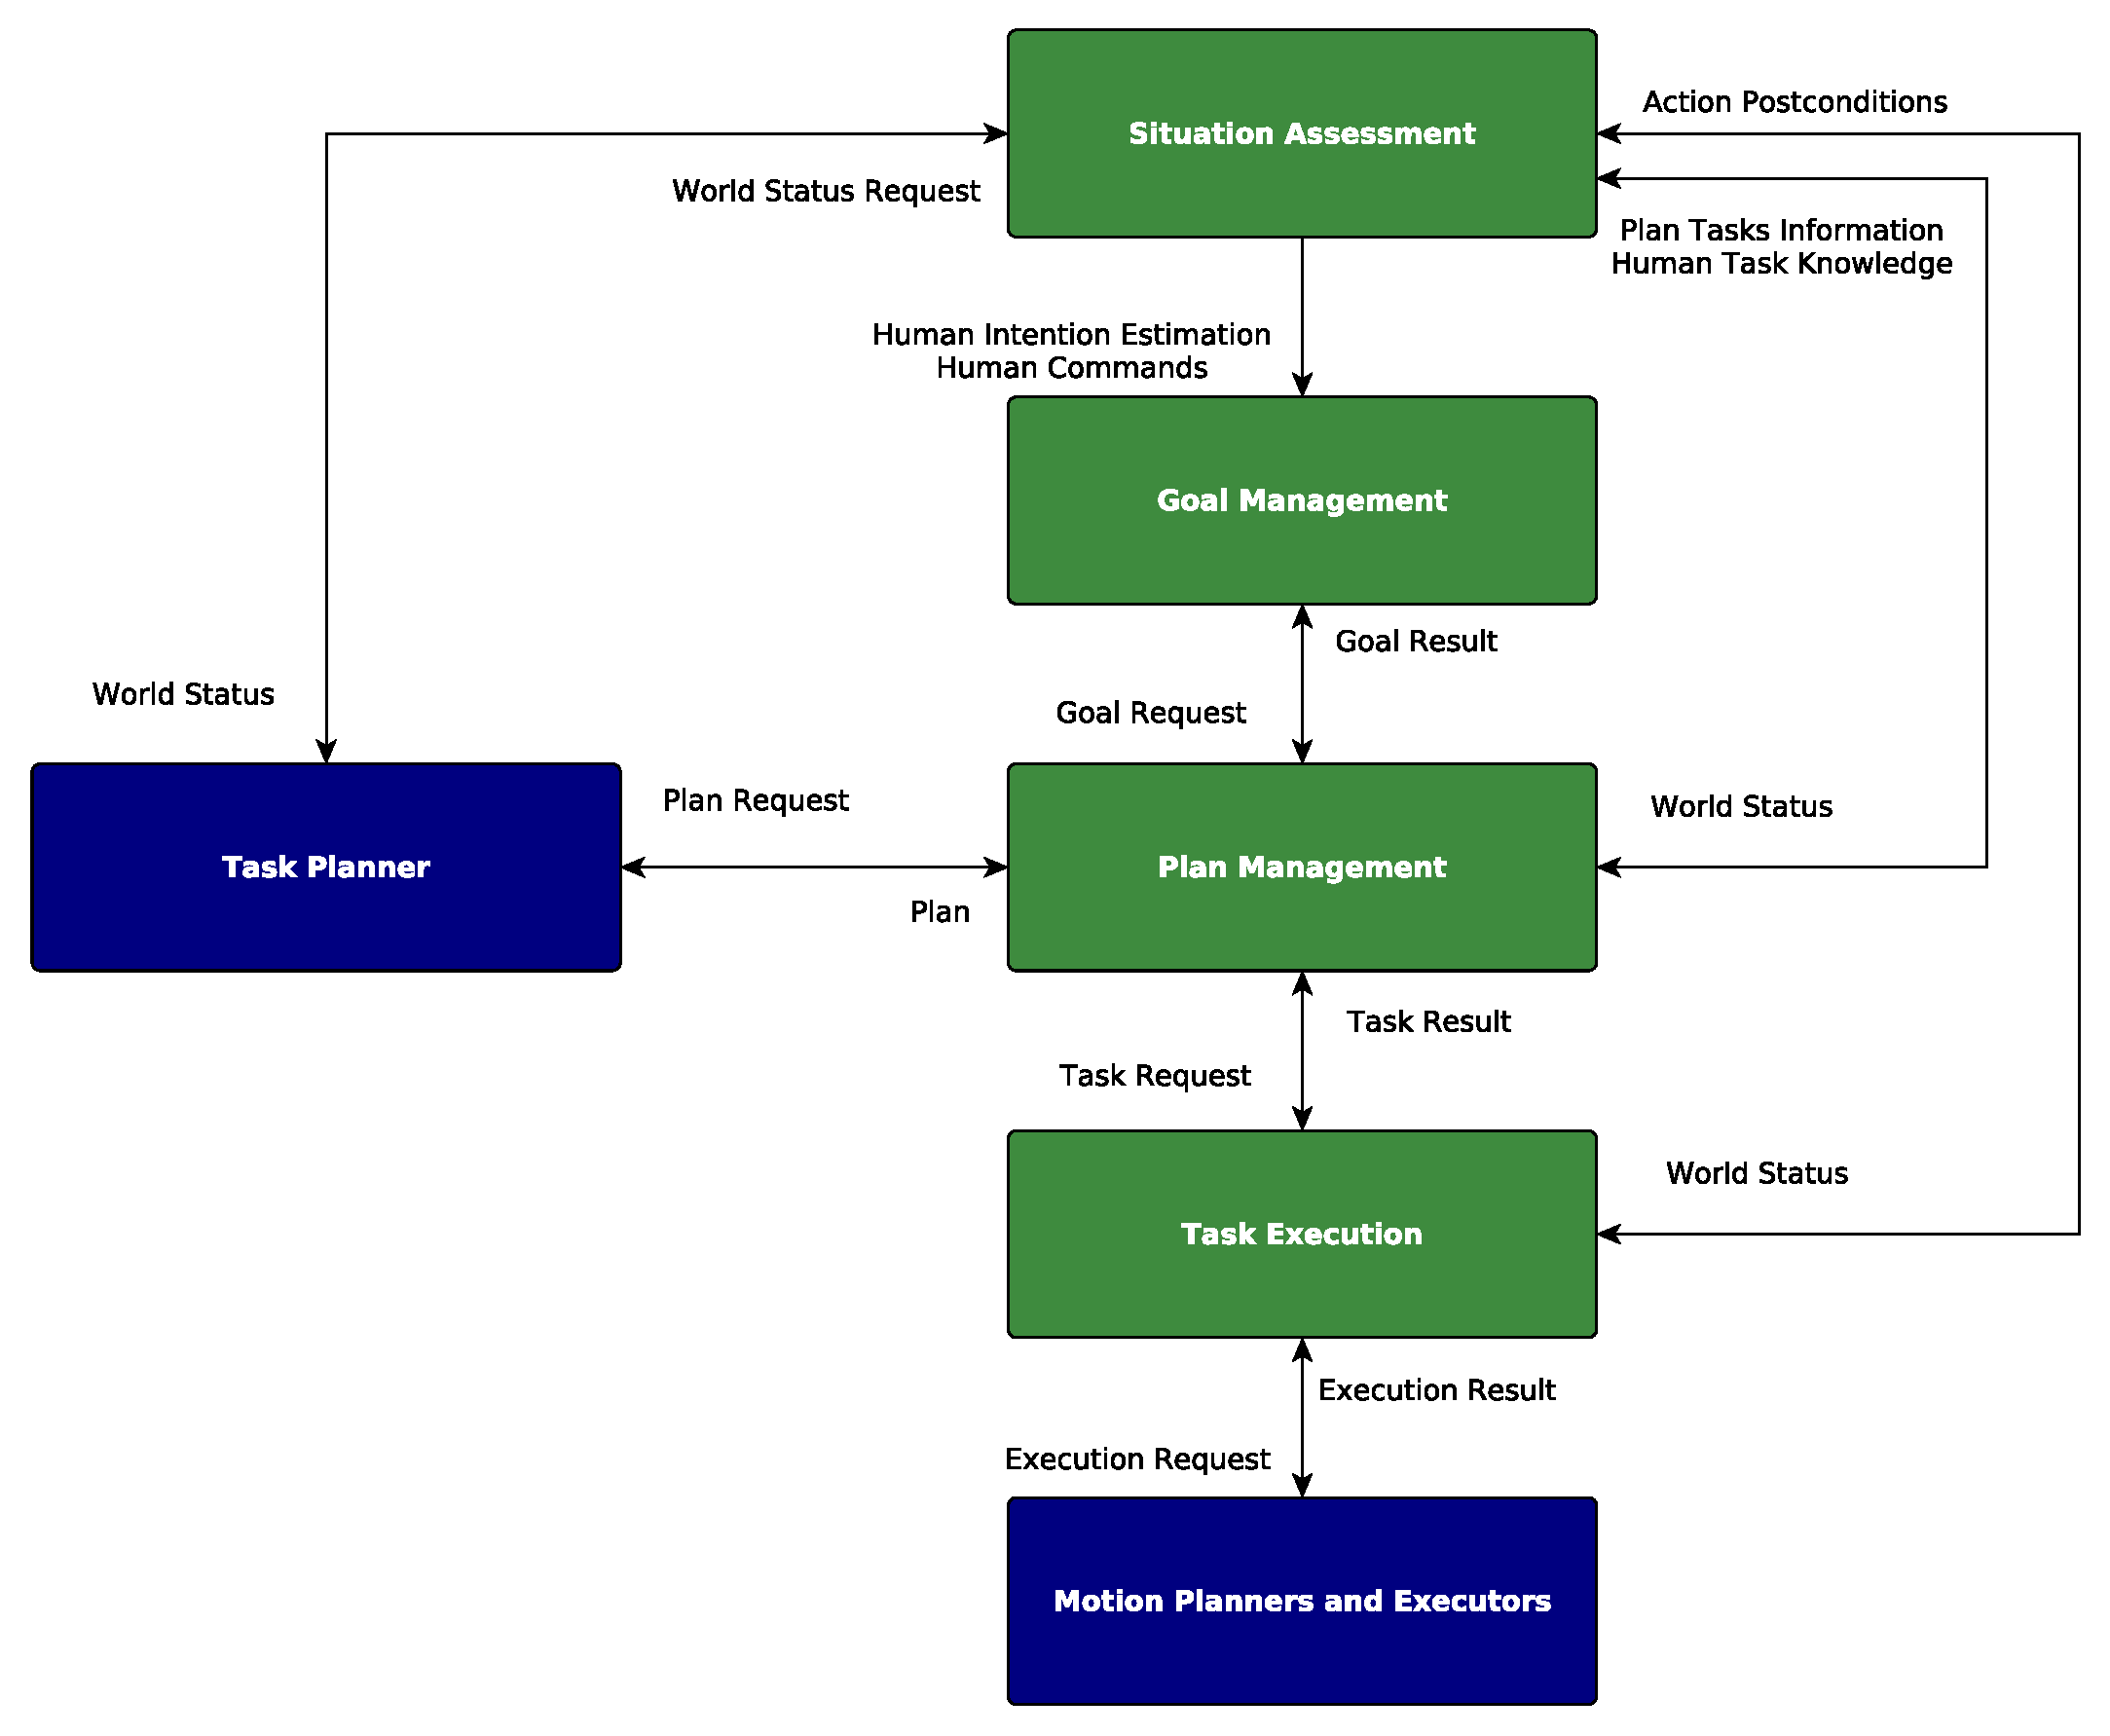
\includegraphics[scale=0.45]{img/intro/system_architecture.pdf}
	\caption[System architecture]{This picture shows the different layers of the system.}
	\label{fig:intro-system_architecture}
\end{figure}

The system also easily interface with different modules, which can be changed depending on the current needs:
\begin{itemize}
\item Task Planner. The Plan Production and Management layer provides an interface for different planners. New planners can be introduced by creating a bridge that respects the interface provided by the provided interface.
\item Motion Planners and Executors. The Execution Management layers is interfaced with a set of motion planners and an executor to accomplish the robot's movements and actions. New modules can be introduced by respecting the interface used in the layer.
\end{itemize}

\section{Organization of the Thesis}
This thesis is organized in several chapters. \ref{chapter:situation_assessment} discusses the Situation Assessment Layer, introducing its functionalities and a study to assess a part of its capacities. \ref{chapter:goal_management} shows how our system is able to receive, generate, and manage goals. \ref{chapter:plan_management} analyzes the capacity of our system to produce and manage plans. We discuss two different planners introduced in our system, and the process to explain, negotiate, and adapt plans to users. Finally, we present several plan management algorithms, with different characteristics. \ref{chapter:plan_execution} shows how our system is able to support action executed single-handedly by the robot, as well as our framework to execute joint actions with a human partner. \ref{chapter:case_study} presents two different applications where we used our system: a domestic robot helper and an airport guide. Finally, "introduce conclusion", concludes this work, discussing several possible future extensions. 

\section{Published Works}
\begin{itemize}
\item Milliez, Grégoire, et al. ``Simulating human-robot interactions for dialogue strategy learning." Simulation, Modeling, and Programming for Autonomous Robots. Springer International Publishing, 2014. 62-73.
\item Triebel, Rudolph, et al. ``SPENCER: A socially aware service robot for passenger guidance and help in busy airports.", 2015.
\item Fiore, Michelangelo, et al. ``An Adaptive and Proactive Human-Aware Robot Guide." Social Robotics. Springer International Publishing, 2015. 194-203.
\item Fiore Michelangelo, et al. ``On planning and task achievement modalities for human-robot collaboration." Experimental Robotics. Springer International Publishing, 2016.
\item Milliez, Grégoire, et al. ``Using human knowledge awareness to adapt collaborative plan generation, explanation and monitoring." The Eleventh ACM/IEEE International Conference on Human Robot Interation. IEEE Press, 2016.
\item Devin, Sandra et al. ``Some essential skills and their combination in an architecture for a cognitive and interactive" robot arXiv preprint arXiv:1603.00583, 2016
\item Caccavale, Riccardo, et al. ``Attentional Supervision of Human-Robot Collaborative Plans." The IEEE International Symposium on Robot and Human Interactive Communication (RO-MAN), 2016.
\end{itemize}
% Chapter Template

\chapter{Situation Assessment} % Main chapter title

\label{chapter-situation_assessment} % Change X to a consecutive number; for referencing this chapter elsewhere, use \ref{ChapterX}

\lhead{Chapter . \emph{Situation Assessment}} % Change X to a consecutive number; this is for the header on each page - perhaps a shortened title

In this chapter we introduce the Situation Assessment capacities of our system. 

%TODO: Citations on Toaster 
\section{Introduction}
\label{situation_assessment-intro}
%Motivation
For any application that's not repetitive, control based, it's necessary that robots have a representation of their environment. Depending on the application, these information could be simple or more complex. Imagine, for example, a robot that needs to clean the floor of a room. A simple implementation of this idea would rely on a map of the room and laser or bumper sensors to avoid or detect obstacles. Now, imagine a household robot that needs to actively help a family that lives in an apartment, by fetching objects, providing information and help accomplish various tasks. Clearly, in this situation, the robot needs a deeper degree of reasoning on sensor data: laser points and camera images need to be integrated to recognize objects and humans, spatial relationships between objects (e.g. the cup is on the table) and humans (e.g. the human has the cup) need to be properly modeled, actions performed by humans, and their effects on the environment, need to be recognized, and so on.

%What is situation assessment
In this situation, there is a need for a module that performs different kind of reasoning on perceptual data, and produces information that can be used by the rest of the system. Maintaning knowledge and understanding of the current situation, also known as situation awareness, is called situation assessment. 
Endsley in \cite{endsley1995} explains that "situation awareness incorporates an operator's understanding of the situation as a whole, forming the basis for decision making".


\subsection{Situation Assessment}
%what are people doing with situation assessment and belief management
A variety of robotic systems have made a situation assessment component to fit the need of the robot in a particular task application. In \cite{beck2011}, the situation assessment system is based on Dynamic Markov chains to model the environment states and their evolution. It presents an application for a mobile robot to navigate in a narrow passage.
\cite{Chella2010} aims to build a "higher order" perception, giving the robot the ability to reason on its own inner world.
\cite{Kluge01situationassessment} presents an empirical assessment of situations for a mobile robot in a crowded public environment applied to recognize situations of deliberate obstruction. In our situation assessment software we focus on what is represented (human, objects ...) and we support heterogeneous type of sensors and data to provide a semantic interpretation of the environment with the aim to have a situation assessment capability that can be used in a various set of applications (see \ref{sec:applications}).


\subsection{Theory of Mind}
%A Geometric
perceptual perspective taking, whereby 
human can understand that other people have a different  perception of the world, and 2) 
conceptual perspective taking, whereby humans can go further and attribute beliefs and feelings to other people~\cite{Baron1985}.

Understanding properly others' intention requires to reason about their beliefs and thoughts, and on how they affect actions. This skill is called Theory of Mind \cite{premack1978does}. An ability linked to this concept is perspective taking, which is widely studied in developmental literature.  Flavell in \cite{flavell1977development} describes two levels of perspective taking: 
1) perceptual perspective taking, whereby  humans can understand that other people see the world differently~\cite{Tversky1999}, and 2) conceptual perspective taking, whereby humans can go further and attribute thoughts and feelings to other people~\cite{Baron1985}. Studies on individuals that don't possess the required mechanisms to perform perspective taking, like young children \cite{frick2014picturing}, 
have put into light the difficulties these people have to accomplish everyday social relationships and confirmed the importance of this ability.

Previous works in robotics have shown that enhancing the robot's perspective taking abilities improves its reasoning capabilities, leading to more appropriate and efficient task planning and interaction strategies \cite{breazeal2006,Trafton2005,ros2010one}.

Concerning level two, various research on human robot interaction already aim to represent the human belief state.
Breazal et al.~\cite{BreazealGB09} proposed one of the first human-robot implementation. In our previous work \cite{Milliez2014}, we made a primitive implementation to solve the Sally and Anne test described by Wimmer in~\cite{Wimmer1983}. In this primitive implementation, the reasoning on others belief state was limited to object position. We propose here a more generic approach to represent any kind of belief the human may hold on the environment.
%B conceptual

The first point we need to introduce is the concept of intention. There are many different definitions of intention in psychology \cite{bruner1981} and philosophy \cite{bratman1984} literature. In this paper we define an intention as the wish and will to achieve a goal. The intention emerges from contextual causes (motivations) and is present 

An important study linked to conceptual perspective taking is the 'divergent belief task'.  Formulated in~\cite{wimmer1983}, this kind of task requires the ability to recognize that others can have beliefs about the world that differ from the observable reality. ~\cite{BreazealGB09} proposed one of the first human-robot implementations, resulting in more advanced goal recognition skills. This is a primary issue of intention recognition, since, as explained by \cite{byom2013theory} "as humans, we generally believe that others act in ways that are consistent with their beliefs and goals".


Also, the authors's belief modeling (described fully in \cite{briggs2011facilitating}) is oriented toward communication problems and not geometrical and spatial perspective taking issues.

\subsection{Activity Recognition}

The recognition of human activities is an important topic in computer science research, which can be studied at different levels. Anticipating human actions and movements allows the robot to adapt its behavior and proactively help humans, as studied in \cite{koppula2013anticipating}. An interesting idea is using the robot's own internal models in order to recognize actions and predict user intents, as shown by the \textit{HAMMER} system in \cite{demiris2007prediction}. Sequences of actions can be linked to plans, a well-known topic called plan recognition. Several approaches have been studied in this domain using, for example, classical planning \cite{ramirez2009plan}, probabilistic \cite{bui2003general} or logic techniques \cite{singla2011abductive}. An interesting framework for intention recognition is the Bayesian Theory of Mind \cite{baker2014modeling}, used to represent the inference process of an observer looking at another agent's behaviors, with POMDPs and Dynamic Bayesian Networks (DBNs). 

Two approaches that can be used for intention estimation are Interactive Partially Observed Markov Decision Processes (I-POMDP) and Inverse Learning. I-POMDP  \cite{gmytrasiewicz2004interactive} offer a rich framework that extends Partially Observed Markov Decision Processes (POMDP) in a multi-agent setting. Inference in these models can be extremely complex, but there have been attempts at solving this issue, like in \cite{doshi2009monte,hoang2013interactive}. 

Inverse Reinforcement Learning \cite{ng2000algorithms} formulates the problem of computing an unknown reward function of an agent after observing his behavior. This strategy has been applied, with Bayesian Networks (BN), in \cite{Nagai2015}, in order to learn the mental model of another agent, and choose appropriate actions for a relationship building task. A linked approach is inverted planning, which has been applied in a bayesian framework in \cite{baker2009action}  for human action understanding.

Contextual information can be used to further disambiguate complex situations. \cite{Liu2014} shows a system using BNs to understand users' intentions with an emphasis on contextual information.

\section{Definitions}
%Fact
%Action


\section{Situation Assessment}
\label{situation_assessment-situation_assessment}
\subsection{Entity Recognition}


\section{Belief Management}
\label{situation_assessment-belief_management}

\section{Action and Intention Inference}
\label{situation_assessment-intention_recognition}

\subsection{Intention Graph}
\subsection{Context to Intentions}
\subsection{Intentions to Actions}
\subsection{Actions to Observations}
\subsection{Inference Process}

\section{Experiments}
\label{situation_assessment-experiments}
\subsection{Case Study}
\subsection{Robot Implementation}
\subsection{Discussion}

%%refine better when writing... basically it's that paper. Maybe we can put something novel? Like a better study


%\bibliographystyle{plainnat} % Use the "unsrtnat" BibTeX style for formatting the Bibliography
\bibliographystyle{apalike}
%\bibliographystyle{unsrtnat}
\lhead{\emph{Bibliography}} % Change the page header to say "Bibliography"
%\bibliography{thesis} % The references (bibliography) information are stored in the file named "thesis.bib"

\newpage
\appendix
\end{document}  